\chapter{Neural Network Design}
\section{Introduction}
The robot controls its motors using the artificial neural networks and the deep deterministic policy gradient (DDPG) algorithm, produced by Lillicrap et al. The system runs in Python 3, leaning heavily on the TensorFlow library.

\section{Reinforcement Learning Concepts}
Reinforcement learning (RL) is a subset of machine learning that aims to solve control and action selection problems rather than to perform classification or data clustering. Most reinforcement learning problems involve six main elements: an actor, the environment, rewards, a policy, a value function, and sometimes a model. An actor (sometimes called an agent) takes actions in an environment which returns a state and reward, illustrated in Figure \ref{fig:actor_env_loop}. The actor's primary goal is to maximize the accumulated reward received from the environment. A policy determines which actions the actor takes given the current state and can be considered a mapping from state to action. The value function indicates the long-term reward expected from a state so even if a state only has a small immediate reward, it may possess high value since it leads to high reward states. Some algorithms involve a model of the environment, allowing prediction of the next state from the current state and action.
\begin{figure}[H]   % [h] means here
	\centering 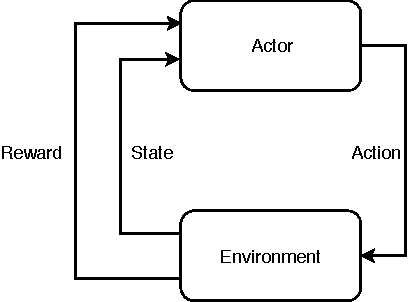
\includegraphics[width=3in, height=3.85in, keepaspectratio]{figures/actor_env_loop.pdf}
	\caption{Actor-Environment Feedback Loop}\label{fig:actor_env_loop}
\end{figure}

long-term discounted reward: $G_t$.
\begin{equation}
	G_t=R_{t+1}+\gamma R_{t+2}+\gamma^2 R_{t+3} + \dots = \sum_{k=0}^{\infty} \gamma^k R_{t+k+1}
\end{equation}
The discount factor $\gamma$ weights the worth of future rewards exponentially by their distance into the future. It ranges from 0 to 1 where 0 makes future rewards worthless while a discount factor of 1 means future rewards are worth their face value now. In practice, the discount factor is less than 1 in order to allow $G_t$ to converge \cite{sutton_2017}.

Table \ref{tab:rl_defs} summarizes some common terms and definitions used in the reinforcement learning literature.

\LTXtable{\textwidth}{tables/tab_rl_defs.tex}

\section{Reinforcement Learning Algorithms}
Many reinforcement learning algorithms have been applied to control including Tabular Q-Learning, State-Action-Reward-State-Action (SARSA), and Deep Deterministic Policy Gradient (DDPG), among others.

RL algorithms can be classified their use of models and actor policy. Model-based strategies first develop a model of the environment and then produce a controller using the model. Model-free algorithms forego An optimal actor chooses actions that maximize the total reward received using a strategy called the optimal policy, $\pi_*$. However, actors do not necessarily .

\subsection{Q-Learning}
Q-Learning is an off-model, off-policy 

\subsection{State-Action-Reward-State-Action (SARSA)}
SARSA is an on-policy algorithm similar which shares many characteristics with Q-Learning.

\subsection{Deep Q Network (DQN)}


\subsection{Deep Deterministic Policy Gradient (DDPG)}





\section{Artifical Neural Network Implementation}

\section{Training}

\section{Testing}

\section{Results}

